\begin{figure*}[!t]
\centering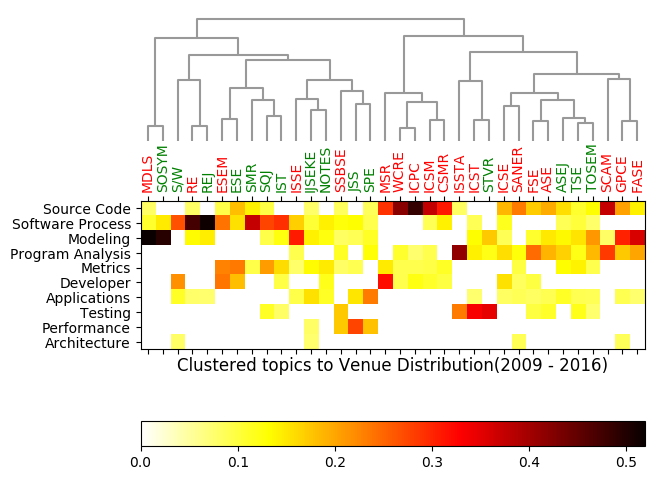
\includegraphics[scale=0.7]{png_heatmap_09_16_dend.png}
\caption{Hierarchical clustering heatmap of 35,000+ 
papers and SE Venues over the last 25 years.
Along the top,  \textcolor{ao(english)}{{\bf green}} denotes
journals and   \textcolor{red}{{\bf red}} denotes  conferences.
Along the left side, the black words are the  topics of \tbl{11topics}. 
Topics are sorted top-to-bottom, most-to-least frequent.
Each cell in the heatmap depicts the 
frequency of a topic in a particular
venue.  The tree diagrams above the venues 
show the results of a bottom up clustering of the venues with respect to the topics. In those clusters, venues are in similar
sub-trees if they have similar pattern of topic frequencies. The venues presented in this figure were selected after much interaction with the international community.
Initially, we started with Google Scholar's list of top venues. 
Next, some 
feedback from reviews of a conference  paper~\cite{Mathew2017}  
made us look more broadly at more conferences and  SE journals.
To that list, using our domain knowledge, we added
venues that we knew were associated with senior researchers in the field;
e.g. the ESEM and SSBSE conferences. 
}
\label{fig:div_heat}
\end{figure*}
